
\documentclass[12pt]{article}
\usepackage[margin=1in]{geometry}


%===============================================================================
%================================== PACKAGES ===================================
%===============================================================================

% For using float option H that places figures 
% exatcly where we want them
\usepackage{float}
% makes figure font bold
\usepackage{caption}
\captionsetup[figure]{labelfont=bf}
% For text generation
\usepackage{lipsum}
% For drawing
\usepackage{tikz}
% For smaller or equal sign and not divide sign
\usepackage{amssymb}
% For the diagonal fraction
\usepackage{xfrac}
% For enumerating exercise parts with letters instead of numbers
\usepackage{enumitem}
% For dfrac, which forces the fraction to be in display mode (large) e
% even in math mode (small)
\usepackage{amsmath}
% For degree sign
\usepackage{gensymb}
% For "\mathbb" macro
\usepackage{amsfonts}
% For positioning 
\usepackage{indentfirst}
\usetikzlibrary{shapes,positioning,fit,calc}
% for adjustwidth environment
\usepackage{changepage}
% for arrow on top
\usepackage{esvect}
% for mathbb 1
\usepackage{bbm}
% for mathsrc
\usepackage[mathscr]{eucal}
% For degree sign
\usepackage{gensymb}
% For quotes
\usepackage{csquotes}
% For vertical lines
\usepackage{mathtools}
% For cols
\usepackage{multicol}

% for tikz
\usepackage{pgfplots}
\pgfplotsset{compat=1.18}
\usepackage{amsmath}
\usepgfplotslibrary{groupplots}


%===============================================================================
%==================================== FONTS ====================================
%===============================================================================


% Mathcal
\newcommand{\acal}{\mathcal{A}}
\newcommand{\bcal}{\mathcal{B}}
\newcommand{\ccal}{\mathcal{C}}
\newcommand{\dcal}{\mathcal{D}}
\newcommand{\ecal}{\mathcal{E}}
\newcommand{\fcal}{\mathcal{F}}
\newcommand{\gcal}{\mathcal{G}}
\newcommand{\hcal}{\mathcal{H}}
\newcommand{\ical}{\mathcal{I}}
\newcommand{\jcal}{\mathcal{J}}
\newcommand{\kcal}{\mathcal{K}}
\newcommand{\lcal}{\mathcal{L}}
\newcommand{\mcal}{\mathcal{M}}
\newcommand{\ncal}{\mathcal{N}}
\newcommand{\ocal}{\mathcal{O}}
\newcommand{\pcal}{\mathcal{P}}
\newcommand{\qcal}{\mathcal{Q}}
\newcommand{\rcal}{\mathcal{R}}
\newcommand{\scal}{\mathcal{S}}
\newcommand{\tcal}{\mathcal{T}}
\newcommand{\ucal}{\mathcal{U}}
\newcommand{\vcal}{\mathcal{V}}
\newcommand{\wcal}{\mathcal{W}}
\newcommand{\xcal}{\mathcal{X}}
\newcommand{\ycal}{\mathcal{Y}}
\newcommand{\zcal}{\mathcal{Z}}

% Mathfrak
\newcommand{\afrak}{\mathfrak{A}}
\newcommand{\bfrak}{\mathfrak{B}}
\newcommand{\cfrak}{\mathfrak{C}}
\newcommand{\dfrak}{\mathfrak{D}}
\newcommand{\efrak}{\mathfrak{E}}
\newcommand{\ffrak}{\mathfrak{F}}
\newcommand{\gfrak}{\mathfrak{G}}
\newcommand{\hfrak}{\mathfrak{H}}
\newcommand{\ifrak}{\mathfrak{I}}
\newcommand{\jfrak}{\mathfrak{J}}
\newcommand{\kfrak}{\mathfrak{K}}
\newcommand{\lfrak}{\mathfrak{L}}
\newcommand{\mfrak}{\mathfrak{M}}
\newcommand{\nfrak}{\mathfrak{N}}
\newcommand{\ofrak}{\mathfrak{O}}
\newcommand{\pfrak}{\mathfrak{P}}
\newcommand{\qfrak}{\mathfrak{Q}}
\newcommand{\rfrak}{\mathfrak{R}}
\newcommand{\sfrak}{\mathfrak{S}}
\newcommand{\tfrak}{\mathfrak{T}}
\newcommand{\ufrak}{\mathfrak{U}}
\newcommand{\vfrak}{\mathfrak{V}}
\newcommand{\wfrak}{\mathfrak{W}}
\newcommand{\xfrak}{\mathfrak{X}}
\newcommand{\yfrak}{\mathfrak{Y}}
\newcommand{\zfrak}{\mathfrak{Z}}

% Mathscr
\newcommand{\ascr}{\mathscr{A}}
\newcommand{\bscr}{\mathscr{B}}
\newcommand{\cscr}{\mathscr{C}}
\newcommand{\dscr}{\mathscr{D}}
\newcommand{\escr}{\mathscr{E}}
\newcommand{\fscr}{\mathscr{F}}
\newcommand{\gscr}{\mathscr{G}}
\newcommand{\hscr}{\mathscr{H}}
\newcommand{\iscr}{\mathscr{I}}
\newcommand{\jscr}{\mathscr{J}}
\newcommand{\kscr}{\mathscr{K}}
\newcommand{\lscr}{\mathscr{L}}
\newcommand{\mscr}{\mathscr{M}}
\newcommand{\nscr}{\mathscr{N}}
\newcommand{\oscr}{\mathscr{O}}
\newcommand{\pscr}{\mathscr{P}}
\newcommand{\qscr}{\mathscr{Q}}
\newcommand{\rscr}{\mathscr{R}}
\newcommand{\sscr}{\mathscr{S}}
\newcommand{\tscr}{\mathscr{T}}
\newcommand{\uscr}{\mathscr{U}}
\newcommand{\vscr}{\mathscr{V}}
\newcommand{\wscr}{\mathscr{W}}
\newcommand{\xscr}{\mathscr{X}}
\newcommand{\yscr}{\mathscr{Y}}
\newcommand{\zscr}{\mathscr{Z}}

% Mathbb
\newcommand{\abb}{\mathbb{A}}
\newcommand{\bbb}{\mathbb{B}}
\newcommand{\cbb}{\mathbb{C}}
\newcommand{\dbb}{\mathbb{D}}
\newcommand{\ebb}{\mathbb{E}}
\newcommand{\fbb}{\mathbb{F}}
\newcommand{\gbb}{\mathbb{G}}
\newcommand{\hbb}{\mathbb{H}}
\newcommand{\ibb}{\mathbb{I}}
\newcommand{\jbb}{\mathbb{J}}
\newcommand{\kbb}{\mathbb{K}}
\newcommand{\lbb}{\mathbb{L}}
\newcommand{\mbb}{\mathbb{M}}
\newcommand{\nbb}{\mathbb{N}}
\newcommand{\obb}{\mathbb{O}}
\newcommand{\pbb}{\mathbb{P}}
\newcommand{\qbb}{\mathbb{Q}}
\newcommand{\rbb}{\mathbb{R}}
\newcommand{\sbb}{\mathbb{S}}
\newcommand{\tbb}{\mathbb{T}}
\newcommand{\ubb}{\mathbb{U}}
\newcommand{\vbb}{\mathbb{V}}
\newcommand{\wbb}{\mathbb{W}}
\newcommand{\xbb}{\mathbb{X}}
\newcommand{\ybb}{\mathbb{Y}}
\newcommand{\zbb}{\mathbb{Z}}


%===============================================================================
%=============================== SPECIAL SYMBOLS ===============================
%===============================================================================


% Orbit (group theory)
\newcommand{\orbit}{\mathcal{O}}
% Normal group
\newcommand{\normal}{\mathcal{N}}
% Indicator function
\newcommand{\indicator}{\mathbbm{1}}
% Laplace transform
\newcommand{\laplace}[1]{\mathcal{L}}
% Epsilon shorthand
\newcommand{\eps}{\varepsilon}
% Omega
\newcommand{\om}{\omega}
\newcommand{\Om}{\Omega}

%===============================================================================
%================================== OPERATORS ==================================
%===============================================================================


% Inverse exponent
\newcommand{\inv}[0]{^{-1}}
% Overline bar
\newcommand{\olsi}[1]{\,\overline{\!{#1}}}
% Less than or equal slanted
\newcommand{\seqs}{\leqslant}
% Greater or equal slanted
\newcommand{\geqs}{\geqslant}
% Subset or equal
\newcommand{\sub}{\subseteq}
% Proper subset
\newcommand{\prosub}{\subset}
% from
\newcommand{\from}{\leftarrow}

% Parantheses
\newcommand{\para}[1]{\left( #1 \right)}
% Curly Braces
\newcommand{\curl}[1]{\left\{ #1 \right\}}
% Brackets
\newcommand{\brac}[1]{\left[ #1 \right]}
% Angled Brackets
\newcommand{\ang}[1]{\left\langle #1 \right\rangle}
% Norm
\newcommand{\norm}[1]{\left\| #1 \right\|}

% Piece wise (use \\ between cases)
\newcommand{\piecewise}[1]{\begin{cases} #1 \end{cases}}

% Bold symbol shorthand
\newcommand{\bl}{\boldsymbol}

% Vertical space
\newcommand{\vs}[1]{\vspace{#1 pt}}
% Horizontal ertical space
\newcommand{\hs}[1]{\hspace{#1 pt}}


%===============================================================================
%============================== TEXT BASED SYMBOLS =============================
%===============================================================================


% Radians
\newcommand{\rad}{\text{rad}}
% Least Common Multiple
\newcommand{\lcm}{\text{lcm}}
% Automorphism
\newcommand{\Aut}{\text{Aut}}
% Variance
\newcommand{\var}{\text{Var}}
% Covariance
\newcommand{\cov}{\text{Cov}}
% Cofactor (matrix)
\newcommand{\cof}{\text{Cof}}
% Adjugate (matrix)
\newcommand{\adj}{\text{Adj}}
% Trace (matrix)
\newcommand{\tr}{\text{tr}}
% Standard deviation
\newcommand{\std}{\text{Std}}
% Correlation coefficient
\newcommand{\corr}{\text{Corr}}
% Sign
\newcommand{\sign}{\text{sign}}

% And text
\newcommand{\AND}{\text{ and }}
% Or text 
\newcommand{\OR}{\text{ or }}
% If text
\newcommand{\IF}{\text{ if }}
% When text
\newcommand{\WHEN}{\text{ when }}
% Then text
\newcommand{\THEN}{\text{ then }}

% 1st
\newcommand{\st}[1]{#1^{\text{st}}}
% 2nd
\newcommand{\nd}[1]{#1^{\text{nd}}}
% 3rd
\newcommand{\rd}[1]{#1^{\text{rd}}}
% nth
\newcommand{\nth}[1]{#1^{\text{th}}}


%===============================================================================
%========================= PROBABILITY AND STATISTICS ==========================
%===============================================================================


% Permutation
\newcommand{\perm}[2]{{}^{#1}\!P_{#2}}
% Combination
\newcommand{\comb}[2]{{}^{#1}C_{#2}}

% Baye's risk
\newcommand{\risk}[1]{\mathscr{R}_{#1}}
% Baye's optimal risk
\newcommand{\riskOptimal}[1]{\mathscr{R}_{#1}^*}
% Baye's empirical risk
\newcommand{\riskEmpirical}[2]{\hat{\mathscr{R}}_{#1}^{#2}}


%===============================================================================
%=================================== CALCULUS ==================================
%===============================================================================


% d over d derivative
\newcommand{\dd}[2]{\dfrac{d#1}{d#2}}
% partial d over d derivative
\newcommand{\partialdd}[2]{\dfrac{\partial #1}{\partial #2}}
% delta d over d derivative
\newcommand{\deltadd}[2]{\dfrac{\Delta #1}{\Delta #2}}

% Integration between a and b
\newcommand{\integral}[4]{\int_{#1}^{#2} #3 \, #4}
% Integration in some space 
\newcommand{\boundIntegral}[2]{\int_{#1} #2 \, d#1}

% Limit
\newcommand{\limit}[3]{\lim_{#1 \to #2} #3}


%===============================================================================
%================================  BIG SYMBOLS  ================================
%===============================================================================


% Sum
\newcommand{\sumof}[2]{\sum_{#1}^{#2}}
% Product
\newcommand{\productof}[2]{\prod_{#1}^{#2}}
% Union
\newcommand{\unionof}[2]{\bigcup_{#1}^{#2}}
% Intersection
\newcommand{\intersectionof}[2]{\bigcap_{#1}^{#2}}
% Or
\newcommand{\orof}[2]{\bigvee_{#1}^{#2}}
% And
\newcommand{\andof}[2]{\bigwedge_{#1}^{#2}}


%===============================================================================
%=============================== LINEAR ALGEBRA ================================
%===============================================================================


% Bold vector arrow
\newcommand{\bv}[1]{\vec{\mathbf{#1}}}

% Matrix or vector (use // for column, & for row) 
% with brackets
\newcommand{\bmat}[1]{\begin{bmatrix} #1 \end{bmatrix}}
% Matrix or vector (use // for column, & for row) 
% with curved brackets
\newcommand{\pmat}[1]{\begin{pmatrix} #1 \end{pmatrix}}
% Matrix or vector (use // for column, & for row) 
% with lines on either side 
\newcommand{\lmat}[1]{\begin{vmatrix} #1 \end{vmatrix}}
% Matrix or vector (use // for column, & for row) 
% with curly braces
\newcommand{\cmat}[1]{\begin{Bmatrix} #1 \end{Bmatrix}}
% Matrix or vector (use // for column, & for row) 
% with no braces
\newcommand{\mat}[1]{\begin{matrix} #1 \end{matrix}}


%===============================================================================
%================================ LARGE OBJECTS ================================
%===============================================================================

% Multiple lines
\newcommand{\multiline}[1]{
\begin{align*}
    #1
\end{align*}
}

% Multiple lines with equation numbers
\newcommand{\eqmultiline}[1]{
\begin{align*}
    #1
\end{align*}
}

% Color
\newcommand{\colorText}[2]{
\begingroup
\color{#1}
    #2
\endgroup
}

% Centered figure
\newcommand{\centerFigure}[2]{
    \begin{figure}[h]
        \centering
            #1
        \caption{#2}
    \end{figure}
}

% Tikz figure
\newcommand{\tikzGraphic}[1]{
    \begin{center}
    \begin{tikzpicture}
        #1
    \end{tikzpicture}
    \end{center}
}

% Enumerate numbers (seperate by \item)
\newcommand{\numbers}{\textbf{\number*)}}

% Enumerate letters (seperate by \item)
\newcommand{\letters}{\textbf{\alph*)}}

\title{%
    \Huge Abstract Algebra \\
    \large by \\
    \Large Dummit and Foote \\~\\
    \huge Part 1: Group Theory \\
    \LARGE Chapter 1: Introduction to Groups \\
    \Large Section 2: Dihedral Groups
}
\date{2023-07-14}
\author{Michael Saba}

\begin{document}
    \pagenumbering{gobble}
    \maketitle
    \newpage
    \setlength{\parindent}{0pt}
    \pagenumbering{arabic}


    \section*{Exercise 1}
    \begin{enumerate}[label=\textbf{\alph*.}]
        \item 
            $|D_6| = 6$
        \item 
            $|D_8| = 8$
        \item 
            $|D_{10}| = 10$
    \end{enumerate}   


    \section*{Exercise 2}
    Proof that for any $x \in D_{2n}$
    and $x \neq r^i$ for any $0 \leqslant i < n$,
    then $rx  =xr^{-1}$: \\
    Since $x \neq r^i$ for $0 \leqslant i < n$,
    then x must be of the form $sr^i$ or $r^is$ where $0 \leqslant i < n$.
    First, we not that $rs = sr^{-1}$. \\
    If $x = sr^i$,
    then we have $rx = rsr^i = sr^-1r^i = sr^{i-1} = sr^{i}r^-1 = xr^{-1}$.
    Likewise, if  $x = r^is$,
    then we have $rx = rr^is = r^{i+1}s = r^{i}rs = r^{i}sr^-1 = xr^{-1}$.


    \section*{Exercise 3}
    Proof that for any $x \in D_{2n}$
    and $x \neq r^i$ for any $0 \leqslant i < n$,
    then $|x| = 2$: \\
    Since $x \neq r^i$ for $0 \leqslant i < n$,
    then x must be of the form $sr^i$ or $r^is$ where $0 \leqslant i < n$.
    First, we not that $rs = sr^{-1}$. \\
    If $x = sr^i$, then
    \[x^2 = sr^isr^i
    = sr^ir^{-1}sr^{i-1}
    = sr^ir^{-2}sr^{i-2} ...
    = sr^ir^{-i}s 
    = ss
    = 1\]
    Likewise, for $x = r^is$, then
    \[x^2 = r^isr^is
    = r^{i-1}sr^{-1}r^is
    = r^{i-2}sr^{-2}r^is ...
    = sr^{-i}r^is 
    = ss
    = 1\]
    So in both cases $|x| \leqslant 2$.
    As $sr^i$ and $r^is$ are not equal to the identity for any $i$,
    then $|x| > 1$,
    so $|x| = 2$.


    \section*{Exercise 4}
    Proof that if $n = 2k$ for $k \in \zbb$,
    and $n \geqslant 4$,
    then $z = r^k$ has order 2,
    and is the only non-identity element of $D_{2n}$
    which commutes with all its other elements: \\
    Since $r^n \in D_{2n}$,
    then $r^n = 1$.
    This means that $r^{2k} = (r^k)^2 = 1$.
    So $|r^k| \leqslant 2$,
    and $r^k \neq 1$,
    which means that $|r^k| = 2$. \\
    Now take $r^i$ for any $i$.
    We have $zr^i = r^kr^i = r^{k+i} = r^ir^k = r^iz$. \\
    As for $sr^i$,
    we first note that $sr^k = r^{-1}sr^{k-1} 
    = r^{-2}sr^{k-2}
    = r^{-k}s$.
    Since $k = \sfrac{n}{2}$,
    then it is the $180 \degree$ rotation, which means that $r^k = r^{-k}$.
    So $sr^k = r^ks$.
    Multiplying both sides by 
    Now, we can show that $zsr^i = r^ksr^i
    = sr^kr^i
    = sr^{k + i}
    = sr^ir^k
    = sr^iz$.
    Likewise, for $r^is$,
    we can also show that $zr^is = r^kr^is
    = r^kr^is
    = r^{k + i}s
    = r^ir^ks
    = r^isr^k
    = r^isz$.
    Moreover, $r^k$ commutes with any element $r^i$,
    which means that $r^k$ commutes with all elements in $D_{2n}$.
    Since $s$ and any $r^i$ where $r^i \neq r^{-i}$ don't commute,
    and since $s$ and $sr^i$ or $r^is$ don't commute unless $r^i \neq r^{-i}$,
    that makes $r^k$ the only element that commutes with all others
    in $D_{2n}$.


    \section*{Exercise 5 $***$}
    Proof that no $x \in D_{2n}$ where $n \geqslant 3$ and is odd
    commutes with any element but the identity: \\
    We know from exercise 1.1.1.3 that no element in any group with
    an odd order except the identity is its own inverse.
    Before we start, we will prove by induction that $r^is = sr^i$: \\
    \textbf{Basis step:}
    We know that for $n = 1$, $rs = sr^{-1}$. \\
    \textbf{Inductive hypothesis:}
    Assume that for $n = k$ that $r^ks = sr^{-k}$. \\
    \textbf{Inductive step:}
    For $n = k + 1$,
    we have $r^{k+1}s = r^krs = r^ksr^{-1}$ (by the basis step),
    and $r^ksr^{-1} = sr^{-k}r^{-1} = sr^{-(k+1)}$ (by our assumption). \\
    So for a rotation $r^i$ to commute with $s$,
    where all rotations can be represented for $0 \leqslant i < n$,
    we need for it to be its own inverse.
    This is impossible however.
    We know that $|r| = n$, 
    and that $r^i = r^{-i}$ implies that $r^{2i} = 1$.
    Since $i < n$,
    then $2i < 2n$, which is the second largest element to the power of
    which $r$ is equal to the identity.
    Moreover, $2i \neq n$, as n is odd.
    That means that no rotation in $D_{2n}$ can commute with $s$. \\
    We can also show that no elements of the form $sr^i$ or $rs^i$
    commute with $s$.
    This is because $s \cdot sr^i = r^i
    \neq sr^i \cdot s
    = r^{-i}s \cdot s
    = r^{-i}$,
    and $r^i \neq r^{-i}$ for the reasons detailed above.
    Likewise, $s \cdot r^is = s \cdot sr^{-i}
    = r^{-i}
    \neq r^is \cdot s
    = r^i$,
    again for the same reasons.
    This means that no elements but the identity commutes with all others
    elements in $D_{2n}$.


    \section*{Exercise 6}
    Proof that for $x, y \in G$, if $|x| = |y| = 2$, and $t = xy$,
    then $tx = xt^{-1}$: \\
    Since $|x| = |y| = 2$,
    then $x = x^{-1}$ and $y = y^{-1}$.
    So, we have:
    \[tx = xy^{-1}x^{-1} = x(xy)^{-1} = xt^{-1}\].

    
    \section*{Exercise 7}
    Proof that
    $G = \langle a, b \mid a^2 = b^2 = (ab)^n = 1 \rangle$
    where $a = s$ and $b = sr$ gives the presentation for $D_{2n}$: \\
    We need to show that the generators of $G$ can generate those of
    \[D_{2n} = \langle r, s \mid s^2 = r^n = 1, rs = sr^{-1} \rangle\].
    We have $s = a$, and $r = ssr = ab$.
    Next, we need to show that the relations in $D_{2n}$'s presentation
    can be derived from those in $G$. \\
    Since $a^2 = 1$, then for $s = a$,
    we get $s^2 = 1$. \\
    From $(ab)^n = 1$, for $sr = b$,
    we get $(ssr)^n = r^n = 1$. \\
    Finally, for $b^2 = 1$,
    we get $(sr)^2 = srsr = 1$, which means that $sr = r^{-1}s^{-1} = r^{-1}s$.
    Since $sr = r^{-1}s$, then $rs = sr^{-1}$. \\
    Next, we show that the converse is true;
    that the relations in $D_{2n}$ give us the relations in $G$. \\
    Since $s^2 = 1$, then for $a = s$,
    we get $a^2 = 1$. \\
    From $r^n = 1$, for $r = ab$,
    we get $(ab)^n = 1$. \\
    Finally, for $rs = sr^{-1}$,
    we get $aba = aab^{-1}$,
    which implies $aba = b^{-1}$,
    so $ab = b^{-1}a^{-1} = (ab)^{-1}$
    so $(ab)^2 = 1$. \\
    This completes the proof.


    \section*{Exercise 8}
    The \textit{cyclic subrgoup of $D_{2n}$ generated by $r$} is the group
    that contains the elements of the set ${1, r, r^2 ... r^{n-1}}$.
    The order of this group is larger or equal to $n$,
    as all the elements are unique (since $|r| = n$).
    By the division algorithm, for an integer $i$, $i = qn + p$
    where $0 \leqslant p < n$.
    So for any element $r^i \in D_{2n}$ ,
    $r^i = r^{nq + p} = r^{nq}r^p = (r^n)^qr^p = 1^qr^p = r^p$.
    This tells us that all rotations belong to the set described above,
    with $r^{n-1}$ as the last one.
    So the order of the group is smaller or equal to $n$.
    This means that the order of the group must be $n$.
    
    
    \section*{Exercise 9}
    The order of the group of rigid motions in $\rbb^3$ of a tetrahedron is: \\
    First consider the vertices 1 and 2.
    We can send 1 to any of the other 2 vertices on the base by rotating the
    polyhedron around the axis $d_4$, which passes through the center of
    the base. We may also send 1 to the tip of the pyramid by rotating the
    polyehdron around any of the other 3 axes.
    After 1 has been fixed, 2, having to remain adjacent to 1 (as the
    motions are rigid) can now be sent to any of the three adjacent vertices
    using some axis to rotate the polyhedron. Once we do that, the
    remaining vertices will have been fixed. \\
    We can count the number of motions using the multiplication rule:
    1 can be sent to 4 vertices, and 2 can be sent to 3. This means we
    have $4 \times 3 = 12$ rigid motions. 

    % Triangle figure
    \begin{figure}[H]
        \centering
        % figure is a tikz drawing
        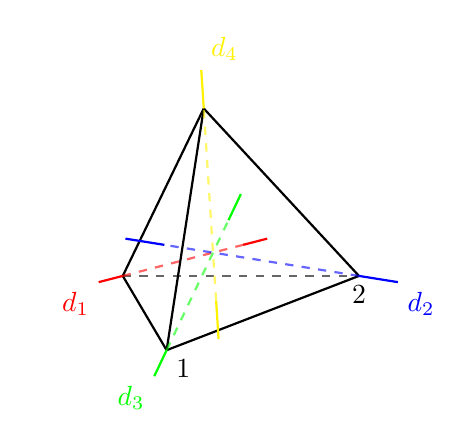
\begin{tikzpicture}[scale=3]
            % Tetrahedron formulae
            \pgfmathsetmacro{\side}{1}
            \pgfmathsetmacro{\halfside}{\side/2}
            \pgfmathsetmacro{\height}{\side * (sqrt(2/3))}
            \pgfmathsetmacro{\halfheight}{\height / 2}
            \pgfmathsetmacro{\altitude}{(\side * sqrt(3)) / 2}
            \pgfmathsetmacro{\extraheight}{0.25}

            % Scope used to shift the coordinates from the basis
            \begin{scope}[shift={(0, 0, 0)}, rotate=0]
                % Triangle base
                \coordinate (A1) at (0, 0, 0);
                \coordinate (A2) at (\side, 0, 0);
                \coordinate (A3) at (\halfside, 0, \height);
                % Triangle tip
                \coordinate (B) at (\halfside, \altitude, \halfheight);
                % Centers of triangles
                \coordinate (C1) at ($1/3*(B) + 1/3*(A2) + 1/3*(A3)$);
                \coordinate (C2) at ($1/3*(B) + 1/3*(A1) + 1/3*(A3)$);                
                \coordinate (C3) at ($1/3*(B) + 1/3*(A1) + 1/3*(A2)$);
                \coordinate (C4) at ($1/3*(A3) + 1/3*(A1) + 1/3*(A2)$);
                % Points aligned with B and C used to draw a symmetry line
                \path (A1) -- (C1) coordinate[pos=-0.2](O1)
                coordinate[pos=1.2](O2);
                \path (A2) -- (C2) coordinate[pos=-0.2](O3)
                coordinate[pos=1.2](O4);
                \path (A3) -- (C3) coordinate[pos=-0.2](O5)
                coordinate[pos=1.2](O6);
                \path (B) -- (C4) coordinate[pos=-0.2](O7)
                coordinate[pos=1.2](O8);

                \node at (O1) [below left, red] {$d_1$};
                \node at (O3) [below right, blue] {$d_2$};
                \node at (O5) [below left, green] {$d_3$};
                \node at (O7) [above right, yellow] {$d_4$};

                \node at (A3) [below right] {$1$};
                \node at (A2) [below] {$2$};

            \end{scope}

            % Draws the coordinate system basis with unit side lengths
            % Is usually transparent, remove to see it for reference
            \begin{scope}[thick, blue, line width=3, opacity=0.4, transparent]
                \draw (0, 0, 0) -- (1, 0, 0);
                \draw (0, 0, 0) -- (0, 1, 0);
                \draw (0, 0, 0) -- (0, 0, 1);   
            \end{scope}

            \begin{scope}[thick]
                \draw (A2) -- (A3) -- (A1);   
                \draw (B) -- (A1) ;
                \draw (B) -- (A2);
                \draw (B) -- (A3);

                \draw [red] (A1) -- (O1);
                \draw [red] (C1) -- (O2);
                \draw [blue] (A2) -- (O3);
                \draw [blue] (C2) -- (O4);
                \draw [green] (A3) -- (O5);
                \draw [green] (C3) -- (O6);
                \draw [yellow] (B) -- (O7);
                \draw [yellow] (C4) -- (O8);
            \end{scope}

            \begin{scope}[thick,dashed,opacity=0.6]
                \draw (A1) -- (A2);
                \draw [red] (A1) -- (C1);    
                \draw [blue] (A2) -- (C2);    
                \draw [green] (A3) -- (C3);  
                \draw [yellow] (C4) -- (B);    
            \end{scope}
        \end{tikzpicture}

        \caption{\label{fig:figure1} Tetrahedron.}
    \end{figure}


    \section*{Exercise 10}
    The order of the group of rigid motions in $\rbb^3$ of a cube is: \\
    First consider the vertices 1 and 2.
    We can send 1 to any of the other 3 vertices on the base square by
    rotating the polyhedron around the axis $d_1$, which passes through
    the center of the square. We may also send 1 to the top square by
    rotating the polyehdron around the other 2 axes (amounting to 8 options).
    After 1 has been fixed, 2, having to remain adjacent to 1 (as the
    motions are rigid) can now be sent to any of the three adjacent vertices
    using some axis to rotate the polyhedron. Once we do that, the
    remaining vertices will have been fixed. \\
    We can count the number of motions using the multiplication rule:
    1 can be sent to 8 vertices, and 2 can be sent to 3. This means we
    have $8 \times 3 = 24$ rigid motions. 


    % Square figure
    \begin{figure}[H]
    \centering
    % figure is a tikz drawing
    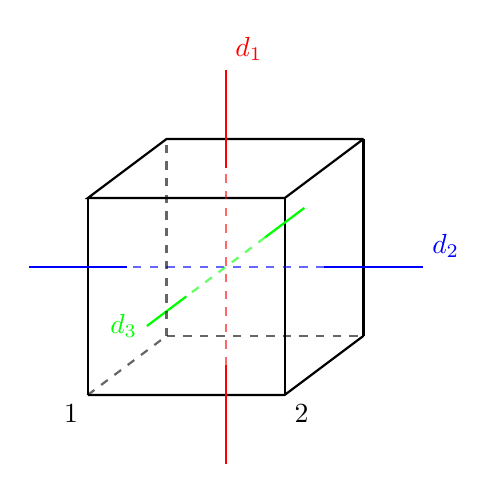
\begin{tikzpicture}[scale=2.5]
        % Cube formulae
        \pgfmathsetmacro{\side}{1}
        \pgfmathsetmacro{\halfside}{\side/2}
        \pgfmathsetmacro{\extra}{0.5}

        % Specifies where the x, y coordinate of the tip of
        % the unite vectors in turn
        \tikzset{
            x={(1cm, 0cm)}, y={(0cm,1cm)}, z={(-0.4cm,-0.3cm)},
        }

        % Scope used to shift the coordinates from the basis
        \begin{scope}[shift={(0, 0, 0)}, rotate=0]
            % Lower square
            \coordinate (A1) at (0, 0, 0);
            \coordinate (A2) at (\side, 0, 0);
            \coordinate (A3) at (\side, 0, \side);
            \coordinate (A4) at (0, 0, \side);
            % Upper square
            \coordinate (B1) at (0, \side, 0);
            \coordinate (B2) at (\side, \side, 0);
            \coordinate (B3) at (\side, \side, \side);
            \coordinate (B4) at (0, \side, \side);
            % Centers of square faces
            \coordinate (C1) at (\halfside, 0, \halfside);
            \coordinate (C2) at (\halfside, \side, \halfside);
            \coordinate (C3) at (\side, \halfside, \halfside);
            \coordinate (C4) at (0, \halfside, \halfside);
            \coordinate (C5) at (\halfside, \halfside, 0);
            \coordinate (C6) at (\halfside, \halfside, \side);
            % Points used in defining symmetry axes 
            \coordinate (D1) at (\halfside, \side + \extra, \halfside);
            \coordinate (D2) at (\halfside, -\extra, \halfside);
            \coordinate (D3) at (\side + \extra, \halfside, \halfside);
            \coordinate (D4) at (-\extra, \halfside, \halfside);
            \coordinate (D5) at (\halfside,  \halfside, - \extra);
            \coordinate (D6) at (\halfside, \halfside, \side + \extra);
            \node at (D1) [above right, red] {$d_1$};
            \node at (D3) [above right, blue] {$d_2$};
            \node at (D6) [left, green] {$d_3$};
            \node at (A3) [below right] {2};
            \node at (A4) [below left] {1};

        \end{scope}

        % Draws the coordinate system basis with unit side lengths
        % Is usually transparent, remove to see it for reference
        \begin{scope}[thick, blue, line width=3, opacity=0.4, transparent]
            \draw (0, 0, 0) -- (1, 0, 0);
            \draw (0, 0, 0) -- (0, 1, 0);
            \draw (0, 0, 0) -- (0, 0, 1);   
        \end{scope}

        \begin{scope}[thick]
            \draw (A2) -- (A3) -- (A4);   
            \draw (B2) -- (A2);
            \draw (B3) -- (A3);
            \draw (B4) -- (A4);
            \draw (B2) -- (B3) -- (B4) -- (B1) -- (B2);   

            \draw [red] (D1) -- (C2);
            \draw [red] (C1) -- (D2);
            \draw [blue] (D4) -- (C4);
            \draw [blue] (C3) -- (D3);
            \draw [green] (D5) -- (C5);
            \draw [green] (C6) -- (D6);
        \end{scope}

        \begin{scope}[thick,dashed,opacity=0.6]
            \draw [red] (C1) -- (C2);   
            \draw [blue] (C3) -- (C4);    
            \draw [green] (C5) -- (C6);    
            \draw (A1) -- (A2);
            \draw (A1) -- (B1);
            \draw (A4) -- (A1);
        \end{scope}
        \end{tikzpicture}

        \caption{\label{fig:figure1} Cube.}
    \end{figure}


    \section*{Exercise 11}
    The order of the group of rigid motions in $\rbb^3$ of an octahedron is: \\
    First consider the vertices 1 and 2.
    We can send 1 to any of the other 4 vertices on the horizontal square by
    rotating the polyhedron around the axis $d_1$, which passes through
    the center of the square. We may also send 1 to the top and bottom vertices
    by rotating the polyehdron around the other 2 axes (amounting to 6 options).
    After 1 has been fixed, 2, having to remain adjacent to 1 (as the
    motions are rigid) can now be sent to any of the four adjacent vertices
    using some axis to rotate the polyhedron. Once we do that, the
    remaining vertices will have been fixed. \\
    We can count the number of motions using the multiplication rule:
    1 can be sent to 6 vertices, and 2 can be sent to 4. This means we
    have $6 \times 4 = 24$ rigid motions. 

    
    % Octahedron figure
    \begin{figure}[H]
    \centering
    % figure is a tikz drawing
    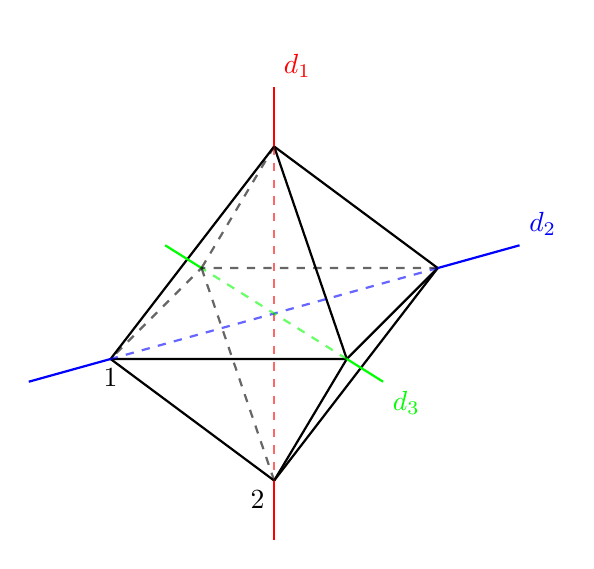
\begin{tikzpicture}[scale=3]
        % Octahedron formulae
        \pgfmathsetmacro{\side}{1}
        \pgfmathsetmacro{\halfside}{\side/2}
        \pgfmathsetmacro{\altitude}{\side/sqrt(2)}
        \pgfmathsetmacro{\extra}{0.25}
        % Scope used to shift the coordinates from the basis
        \begin{scope}[shift={(0, 0, 0)}, rotate=0]
            % Base square
            \coordinate (A1) at (0, 0, 0);
            \coordinate (A2) at (\side, 0, 0);
            \coordinate (A3) at (\side, 0, \side);
            \coordinate (A4) at (0, 0, \side);
            % Upper and lower tips
            \coordinate (B1) at (\halfside, \altitude, \halfside);
            \coordinate (B2) at (\halfside, -\altitude, \halfside);
            % Points used in defining symmetry axes 
            \coordinate (D1) at (\halfside, \altitude + \extra, \halfside);
            \coordinate (D2) at (\halfside, -\altitude -\extra, \halfside);
            \coordinate (D3) at (\side + \extra, 0, -\extra);
            \coordinate (D4) at (-\extra, 0, \side + \extra);
            \coordinate (D5) at (-\extra, 0, -\extra);
            \coordinate (D6) at (\side + \extra, 0, \side + \extra);
            \node at (D1) [above right, red] {$d_1$};
            \node at (D3) [above right, blue] {$d_2$};
            \node at (D6) [below right, green] {$d_3$};

            \node at (A4) [below] {$1$};
            \node at (B2) [below left] {$2$};
        \end{scope}

        % Draws the coordinate system basis with unit side lengths
        % Is usually transparent, remove to see it for reference
        \begin{scope}[thick, blue, line width=3, opacity=0.4, transparent]
            \draw (0, 0, 0) -- (1, 0, 0);
            \draw (0, 0, 0) -- (0, 1, 0);
            \draw (0, 0, 0) -- (0, 0, 1);   
        \end{scope}

        \begin{scope}[thick]
            \draw (A2) -- (A3) -- (A4);  
            \draw (B1) -- (A2);
            \draw (B1) -- (A3);
            \draw (B2) -- (A3);
            \draw (B2) -- (A4);
            \draw (B1) -- (A4);
            \draw (B2) -- (A2); 

            \draw [red] (D1) -- (B1);
            \draw [red] (D2) -- (B2);
            \draw [blue] (D3) -- (A2);
            \draw [blue] (D4) -- (A4);
            \draw [green] (D5) -- (A1);
            \draw [green] (D6) -- (A3);
        \end{scope}

        \begin{scope}[thick,dashed,opacity=0.6]
            \draw [red] (B1) -- (B2);   
            \draw [blue] (A2) -- (A4);  
            \draw [green] (A3) -- (A1);  
            \draw (B2) -- (A1);    
            \draw (B1) -- (A1); 
            \draw (A2) -- (A1) -- (A4);                 
        \end{scope}
        \end{tikzpicture}

        \caption{\label{fig:figure1} Octahedron.}
    \end{figure}


    \section*{Exercise 12}
    The order of the group of rigid motions in $\rbb^3$ of a dodecahedron is: \\
    First consider the vertices 1 and 2.
    We can send 1 to any of the other 5 vertices on its pentagon by
    rotating the polyhedron around the axis $d_6$, which passes through
    the center of said pentagon. We may also send 1 to any other vertex
    by rotating the polyehdron around the other 5 axes (amounting to 20 
    options).
    After 1 has been fixed, 2, having to remain adjacent to 1 (as the
    motions are rigid) can now be sent to any of the three adjacent vertices
    using some axis to rotate the polyhedron. Once we do that, the
    remaining vertices will have been fixed. \\
    We can count the number of motions using the multiplication rule:
    1 can be sent to 20 vertices, and 2 can be sent to 3. This means we
    have $20 \times 3 = 60$ rigid motions. 


    % Dodecahedron figure
    \begin{figure}[H]
        \centering
        % figure is a tikz drawing
        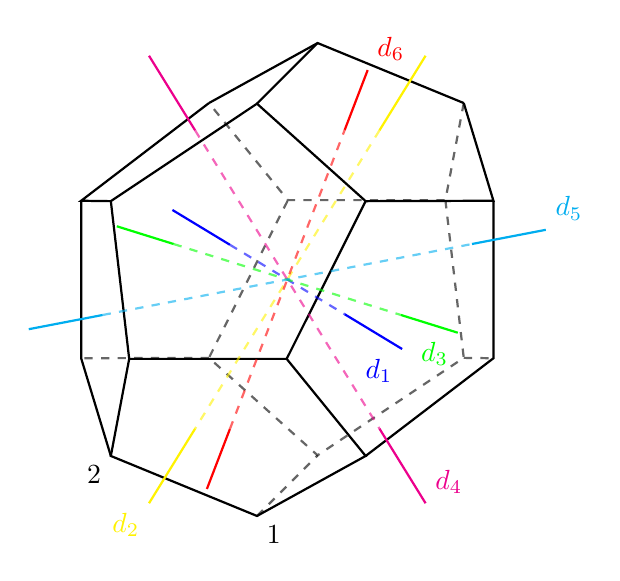
\begin{tikzpicture}[scale=1]
                % Octahedron formulae
        \pgfmathsetmacro{\side}{2}
        \pgfmathsetmacro{\phi}{(1 + sqrt(5))/2}
        % Scope used to shift the coordinates from the basis
        \begin{scope}[shift={(0, 0, 0)}, rotate=0]
            % Base square
            \coordinate (A1) at (0, \phi^2, 1);
            \coordinate (A2) at (0, \phi^2, -1);
            \coordinate (B1) at (\phi, \phi, \phi);
            \coordinate (B2) at (-\phi, \phi, \phi);
            \coordinate (B3) at (\phi, \phi, -\phi);
            \coordinate (B4) at (-\phi, \phi, -\phi);
            \coordinate (C1) at (\phi^2, 1, 0);
            \coordinate (C2) at (-\phi^2, 1, 0);
            \coordinate (D1) at (1, 0, \phi^2);
            \coordinate (D2) at (-1, 0, \phi^2);
            \coordinate (D3) at (1, 0, -\phi^2);
            \coordinate (D4) at (-1, 0, -\phi^2);
            \coordinate (E1) at (\phi^2, -1, 0);
            \coordinate (E2) at (-\phi^2, -1, 0);
            \coordinate (F1) at (\phi, -\phi, \phi);
            \coordinate (F2) at (-\phi, -\phi, \phi);
            \coordinate (F3) at (\phi, -\phi, -\phi);
            \coordinate (F4) at (-\phi, -\phi, -\phi);
            \coordinate (G1) at (0, -\phi^2, 1);
            \coordinate (G2) at (0, -\phi^2, -1);

            % The centers of the bases
            % and a path + offset for a line through both
            \coordinate (Z1) at ($0.2*(A1) + 0.2*(B2) + 0.2*(B1)
            + 0.2*(D2) + 0.2*(D1)$);
            \coordinate (Z2) at ($0.2*(D4) + 0.2*(D3) + 0.2*(F4)
            + 0.2*(F3) + 0.2*(G2)$);
            \path (Z1) -- (Z2) coordinate[pos=-0.5](O1)
            coordinate[pos=1.5](O2);
            
            \coordinate (Z3) at ($0.2*(A1) + 0.2*(A2) + 0.2*(B1)
            + 0.2*(B3) + 0.2*(C1)$);
            \coordinate (Z4) at ($0.2*(E2) + 0.2*(F2) + 0.2*(F4)
            + 0.2*(G1) + 0.2*(G2)$);
            \path (Z3) -- (Z4) coordinate[pos=-0.25](O3)
            coordinate[pos=1.25](O4);

            \coordinate (Z5) at ($0.2*(B4) + 0.2*(D4) + 0.2*(F4)
            + 0.2*(C2) + 0.2*(E2)$);
            \coordinate (Z6) at ($0.2*(B1) + 0.2*(C1) + 0.2*(D1)
            + 0.2*(E1) + 0.2*(F1)$);
            \path (Z5) -- (Z6) coordinate[pos=-0.25](O5)
            coordinate[pos=1.25](O6);

            \coordinate (Z7) at ($0.2*(A2) + 0.2*(A1) + 0.2*(C2)
            + 0.2*(B2) + 0.2*(B4)$);
            \coordinate (Z8) at ($0.2*(G1) + 0.2*(G2) + 0.2*(F3)
            + 0.2*(E1) + 0.2*(F1)$);
            \path (Z7) -- (Z8) coordinate[pos=-0.25](O7)
            coordinate[pos=1.25](O8);

            \coordinate (Z9) at ($0.2*(C2) + 0.2*(E2) + 0.2*(F2)
            + 0.2*(B2) + 0.2*(D2)$);
            \coordinate (Z10) at ($0.2*(B3) + 0.2*(D3) + 0.2*(F3)
            + 0.2*(C1) + 0.2*(E1)$);
            \path (Z9) -- (Z10) coordinate[pos=-0.2](O9)
            coordinate[pos=1.2](O10);

            \coordinate (Z11) at ($0.2*(F2) + 0.2*(D2) + 0.2*(D1)
            + 0.2*(F1) + 0.2*(G1)$);
            \coordinate (Z12) at ($0.2*(A2) + 0.2*(B4) + 0.2*(D4)
            + 0.2*(D3) + 0.2*(B3)$);
            \path (Z11) -- (Z12) coordinate[pos=-0.2](O11)
            coordinate[pos=1.2](O12);

            \node at (O2) [below left, blue] {$d_1$};
            \node at (O4) [below left, yellow] {$d_2$};
            \node at (O6) [below left, green] {$d_3$};
            \node at (O8) [above right, magenta] {$d_4$};
            \node at (O10) [above right, cyan] {$d_5$};
            \node at (O12) [above right, red] {$d_6$};

            \node at (G1) [below right] {1};
            \node at (F2) [below left] {2};

        \end{scope}

        \begin{scope}[thick]    
            \draw (A1) -- (A2);
            \draw (B1) -- (A1) -- (B2);
            \draw (B3) -- (A2) -- (B4);
            \draw (B1) -- (C1) -- (B3);
            \draw (B2) -- (C2) -- (B4);
            \draw (B1) -- (D1) -- (D2) -- (B2);
            \draw (D2) -- (F2) -- (G1) -- (F1) -- (D1);
            \draw (C1) -- (E1) -- (F1);
            \draw (C2) -- (E2) -- (F2);

            \draw [blue] (O1) -- (Z1);
            \draw [blue] (O2) -- (Z2);
            \draw [yellow] (O3) -- (Z3);
            \draw [yellow] (O4) -- (Z4);
            \draw [green] (O5) -- (Z5);
            \draw [green] (O6) -- (Z6);
            \draw [magenta] (O7) -- (Z7);
            \draw [magenta] (O8) -- (Z8);
            \draw [cyan] (O9) -- (Z9);
            \draw [cyan] (O10) -- (Z10);
            \draw [red] (O11) -- (Z11);
            \draw [red] (O12) -- (Z12);
            
        \end{scope}


        \begin{scope}[thick,dashed,opacity=0.6]
            \draw (B3) -- (D3) -- (D4) -- (B4);
            \draw (D3) -- (F3) -- (G2) -- (F4) -- (D4);
            \draw (F3) -- (E1);
            \draw (F4) -- (E2);
            \draw (G1) -- (G2);

            \draw [blue] (Z1) -- (Z2);
            \draw [yellow] (Z3) -- (Z4);
            \draw [green] (Z5) -- (Z6);
            \draw [magenta] (Z7) -- (Z8);
            \draw [cyan] (Z9) -- (Z10);
            \draw [red] (Z11) -- (Z12);
        \end{scope}


        \end{tikzpicture}
        \caption{\label{fig:figure1} Dodecahedron.}
    \end{figure}


    \section*{Exercise 13}
    The order of the group of rigid motions in $\rbb^3$ of an icosahedron is: \\
    First consider the vertices 1 and 2.
    We can send 1 to any of the other 5 vertices on one pentagon by
    rotating the polyhedron around the axis $d_5$, which passes through
    the center of said pentagon. We may also send 1 to any other vertex
    by rotating the polyehdron around the other 5 axes (amounting to 12 
    options).
    After 1 has been fixed, 2, having to remain adjacent to 1 (as the
    motions are rigid) can now be sent to any of the five adjacent vertices
    using some axis to rotate the polyhedron. Once we do that, the
    remaining vertices will have been fixed. \\
    We can count the number of motions using the multiplication rule:
    1 can be sent to 12 vertices, and 2 can be sent to 5. This means we
    have $12 \times 5 = 60$ rigid motions. 


    % Icosahedron figure
    \begin{figure}[H]
        \centering
        % figure is a tikz drawing
        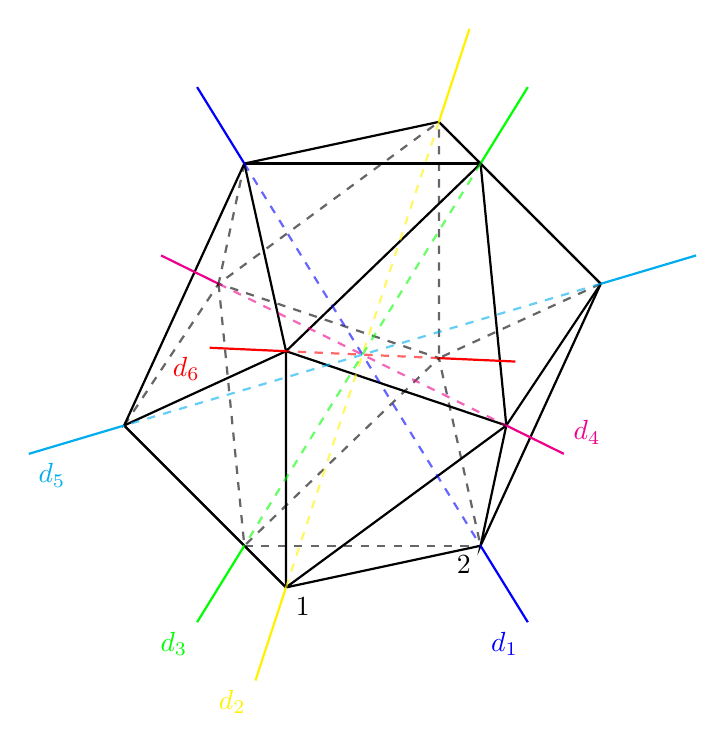
\begin{tikzpicture}[scale=3]

        % Specifies where the x, y coordinate of the tip of
        % the unite vectors in turn
        \tikzset{
            x={(.5cm, 0cm)}, y={(0cm,0.5cm)}, z={(-0.2cm,-0.3cm)},
        }

        % Icosahedron formulae
        \pgfmathsetmacro{\side}{2}
        \pgfmathsetmacro{\phi}{(1 + sqrt(5))/2}
        % Scope used to shift the coordinates from the basis
        \begin{scope}[shift={(0, 0, 0)}, rotate=0]
            \coordinate (A1) at (1, \phi, 0);
            \coordinate (A2) at (-1, \phi, 0);
            \coordinate (B1) at (0, 1, \phi);
            \coordinate (B2) at (0, 1, -\phi);
            \coordinate (C1) at (\phi, 0, 1);
            \coordinate (C2) at (-\phi, 0, 1);
            \coordinate (C3) at (\phi, 0, -1);
            \coordinate (C4) at (-\phi, 0, -1);
            \coordinate (D1) at (0, -1, \phi);
            \coordinate (D2) at (0, -1, -\phi);
            \coordinate (E1) at (1, -\phi, 0);
            \coordinate (E2) at (-1, -\phi, 0);

            % Lines passing through opposite vertices
            \path (A2) -- (E1) coordinate[pos=-0.2](O1)
            coordinate[pos=1.2](O2);
            \path (B2) -- (D1) coordinate[pos=-0.2](O3)
            coordinate[pos=1.2](O4);
            \path (A1) -- (E2) coordinate[pos=-0.2](O5)
            coordinate[pos=1.2](O6);
            \path (C4) -- (C1) coordinate[pos=-0.2](O7)
            coordinate[pos=1.2](O8);
            \path (C3) -- (C2) coordinate[pos=-0.2](O9)
            coordinate[pos=1.2](O10);
            \path (D2) -- (B1) coordinate[pos=-0.5](O11)
            coordinate[pos=1.5](O12);

            \node at (O2) [below left, blue] {$d_1$};
            \node at (O4) [below left, yellow] {$d_2$};
            \node at (O6) [below left, green] {$d_3$};
            \node at (O8) [above right, magenta] {$d_4$};
            \node at (O10) [below right, cyan] {$d_5$};
            \node at (O12) [below left, red] {$d_6$};

            \node at (E1) [below left] {2};
            \node at (D1) [below right] {1};
        \end{scope}

        % Draws the coordinate system basis with unit side lengths
        % Is usually transparent, remove to see it for reference
        \begin{scope}[thick, blue, line width=3, opacity=0.4, transparent]
            \draw (0, 0, 0) -- (1, 0, 0);
            \draw (0, 0, 0) -- (0, 1, 0);
            \draw (0, 0, 0) -- (0, 0, 1);   
        \end{scope}

        \begin{scope}[thick]
            \draw (A1) -- (A2);
            \draw (A1) -- (B2) -- (A2);
            \draw (A1) -- (B1) -- (A2);
            \draw (B1) -- (C1);
            \draw (A1) -- (C1);
            \draw (A1) -- (C3) -- (C1);
            \draw (C1) -- (E1) -- (C3);
            \draw (A2) -- (C2) -- (B1);
            \draw (C1) -- (D1) -- (B1);
            \draw (C2) -- (D1) -- (E1);
            \draw (C2) -- (E2) -- (D1);

            \draw [blue] (O1) -- (A2);
            \draw [blue] (O2) -- (E1);
            \draw [yellow] (O3) -- (B2);
            \draw [yellow] (O4) -- (D1);
            \draw [green] (O5) -- (A1);
            \draw [green] (O6) -- (E2);
            \draw [magenta] (O7) -- (C4);
            \draw [magenta] (O8) -- (C1);
            \draw [cyan] (O9) -- (C3);
            \draw [cyan] (O10) -- (C2);
            \draw [red] (O11) -- (D2);
            \draw [red] (O12) -- (B1);
        \end{scope}

        \begin{scope}[thick,dashed,opacity=0.6] 
            \draw (C3) -- (B2);
            \draw (C3) -- (D2) -- (B2);
            \draw (A2) -- (C4) -- (B2);
            \draw (C2) -- (C4) -- (D2) -- (E1);
            \draw (C4) -- (E2) -- (D2);
            \draw (E2) -- (E1);

            \draw [blue] (A2) -- (E1);
            \draw [yellow] (B2) -- (D1);
            \draw [green] (A1) -- (E2);
            \draw [magenta] (C4) -- (C1);
            \draw [cyan] (C3) -- (C2);
            \draw [red] (D2) -- (B1);
        \end{scope}
        \end{tikzpicture}

        \caption{\label{fig:figure1} Icosahedron.}
    \end{figure}


    \section*{Exercise 14}
    The set of generators of the additive group $(\zbb, +)$ includes just 
    1 since any number can be represented as a sum of 1 and $-1$s.


    \section*{Exercise 15}
    The set of generators of the additive group $(\zbb/n\zbb, +)$ includes just 
    $\olsi{1}$ since the modulo classes are all positive, and can be
    represented by a sum of $\olsi{1}$s or lack thereof.


    \section*{Exercise 16}
    Proof that for $G = \langle a, b \mid a^2 = b^2 = (ab)^2 = 1 \rangle$,
    if we take $a = r$ and $b = s$,
    then $G$ is the dihedral group $D_4$: \\
    If we consider $a = r$ and $b = s$,
    trivially, the generators of $G$ give us the generators of $D_4$.
    Moreover, for $D_{2n} = D_4$, $n = 2$. \\
    To show the relations in $D_4$ give us $G$'s relations,
    we note that since $r^n = r^2 = 1$,
    then $a^2 = 1$,
    and since $s^2 = 1$,
    then $b^2 = 1$.
    Finally, as $rs = sr^{-1}$,
    then $ab = ba^{-1}$.
    Since $a^2 = 1$, $a^{-1} = a$.
    So $ab = ba$, meaning $a$ and $b$ commute.
    So $(ab)^2 = abab = aabb = a^2b^2 = 1 \cdot 1 = 1$. \\ 
    Conversely, if we start with $G$'s relations,
    then we have $a^2 = 1$,
    so $r^2 = r^n = 1$,
    and since $b^2 = 1$,
    then $s^2 = 1$.
    Finally, as $(ab)^2 = abab = 1$,
    we have $abab = 1$, so $ab = b^{-1}a^{-1}$.
    Since $b^2 = 1$, $b^{-1} = b$,
    so $ab = ba^{-1}$,
    which means that $rs = sr^{-1}$. \\
    This completes the proof.


    \section*{Exercise 17}
    For $X_{2n} = \langle x, y \mid x^n = y^2 = 1, xy = yx^2 \rangle$: \\
    \begin{enumerate}[label=\textbf{\alph*.}]
        \item 
            Proof that if $n = 3k$, then $|X_{2n}| = 6$
            and that if we consider $x = r$ and $y = s$,
            then $X_{2n}$ can be shown to have the same generators and 
            relations as $D_6$: \\
            First we have $xy = yx^2
            \implies xy^2 = yx^2y = yxyx^2$,
            so $yxyx^2 = yyx^2x^2 \implies
            x^4 = x
            \implies x^3 = 1
            \implies x^2 = x^{-1}$.
            So $x^3 = y^2 = 1$ and $xy = yx^{-1}$.
            Since we took $x = r$ and $y = s$,
            then the generators and relations of $X_{2n}$ give us the
            generators and relations of $D_6$ where $k = 1$. \\
            We can also show that $D_6$'s relations give us $X_{2n}$'s:
            Since $s^2 = 1$, then $y^2 = 1$.
            Likewise, since $r^n = r^3 = 1$,
            if we take $k = 1$,
            then $x^{3k} = x^n = 1$.
            Finally, since $x^3 = 1$, $x^2 = x^{-1}$,
            then $rs = sr^{-1}$ implies $xy = yx^{2}$.
            So $X_{2n} = D_6$,
            which means that $|X_{2n}| = |D_6| = 6$.
        \item 
            Proof that we have $x = 1$ and $|X_{2n}| = 2$
            if $gcd(3, n) = 1$: \\
            From the last part, we know that $x^3 = 1$.
            However, as $gcd(3, n) = 1$, $n$ shares no factors with 3,
            so $n \neq 3k$ where $k \in \zbb$.
            So $n \equiv 1 \mod 3$ or $n \equiv 2 \mod 3$. 
            Which means that for some $p, q \in \zbb$,
            $n = 3p + 1$ or $n = 3q - 1$. \\
            If $n = 3p + 1$, $x^{3p + 1} = 1$,
            so $x^{3p}x = (x^3)^px = 1^px = x = 1$. \\
            Otherwise, if $n = 3q - 1$, $x^{3q - 1} = 1$,
            so $x^{3q}x^{-1} = (x^3)^qx^{-1} = 1^qx^{-1} = x^{-1} = 1$.
            So $x = 1$ (since $1 \cdot 1 = 1$). \\
            So $X_{2n} = \{1, y\}$,
            which means that $|X_{2n}| = 2$.
    \end{enumerate}   

    \section*{Exercise 18 $***$}
    For $Y = \langle u, v \mid u^4 = v^3 = 1, uv = v^2u^2 \rangle$:
    \begin{enumerate}[label=\textbf{\alph*.}]
        \item 
            $v^3 = 1$, so $v^2 = v^{-1}$.
        \item 
            We have $v^2u^3v = (v^2u^2)(uv) = uvv^2u^2 = uv^3u^2 = u^3$.
            So $v^2u^3v = u^3$,
            hence $vv^2u^3v = vu^3$,
            which implies that $v^3u^3v = vu^3$,
            so $ u^3v = vu^3$.
        \item 
            $u^4 = 1$, so $u^8 = 1$, so $u^9 = u$.
            So $u^9v = u^6u^3v = u^6vu^3 = u^3vu^6 = vu^9 = vu$.
            So $uv = vu$.
        \item 
            We know that $uv = v^2u^2$ and $uv = vu$,
            so $vu = v^2u^2$.
            Hence $uv = vu = v^{-1}v^2u^2u^{-1} = v^{-1}vuu^{-1} = 1$.
        \item 
            $uv = 1$ and $u4v^3 = 1$.
            So $u^3uvv^2 = 1$,
            which implies that $u^3v^2 = 1$,
            hence $u^2uvv = 1$.
            This tells us that $u^2v = 1$,
            so $uuv = 1$,
            so $u = 1$.
            Since $1 = uv = 1v$, 
            then $v = 1$. \\
            We conclude that since $u$ and $v$ are $Y$'s generators,
            $Y = {1}$ (the \textit{trivial group}).

    \end{enumerate}   


\end{document}